\documentclass{standalone}


\usepackage{../core}

\begin{document}

\begin{tikzpicture}[
  scale=1.5,
  >=latex,
  NS/.style={draw=col1dark,text=black,fill=col1dark,inner sep=0,fill opacity=0,text opacity=1,font=\normalsize,line width=1.5pt,minimum width=9.3em,minimum height=7em,rounded corners=0pt,font=\sffamily},
  LL/.style={->,line width=1.5pt,color=col1dark,line cap=round}
  ]

  \node[draw=col1dark,line width=1.5pt,inner sep=8pt] (f) at (2.8,3) {\large\sffamily Investigate the use of sampling to perform approximate inference in PSMs};
  
  \node[NS] (a) at (0,0) {\begin{minipage}{8.5em}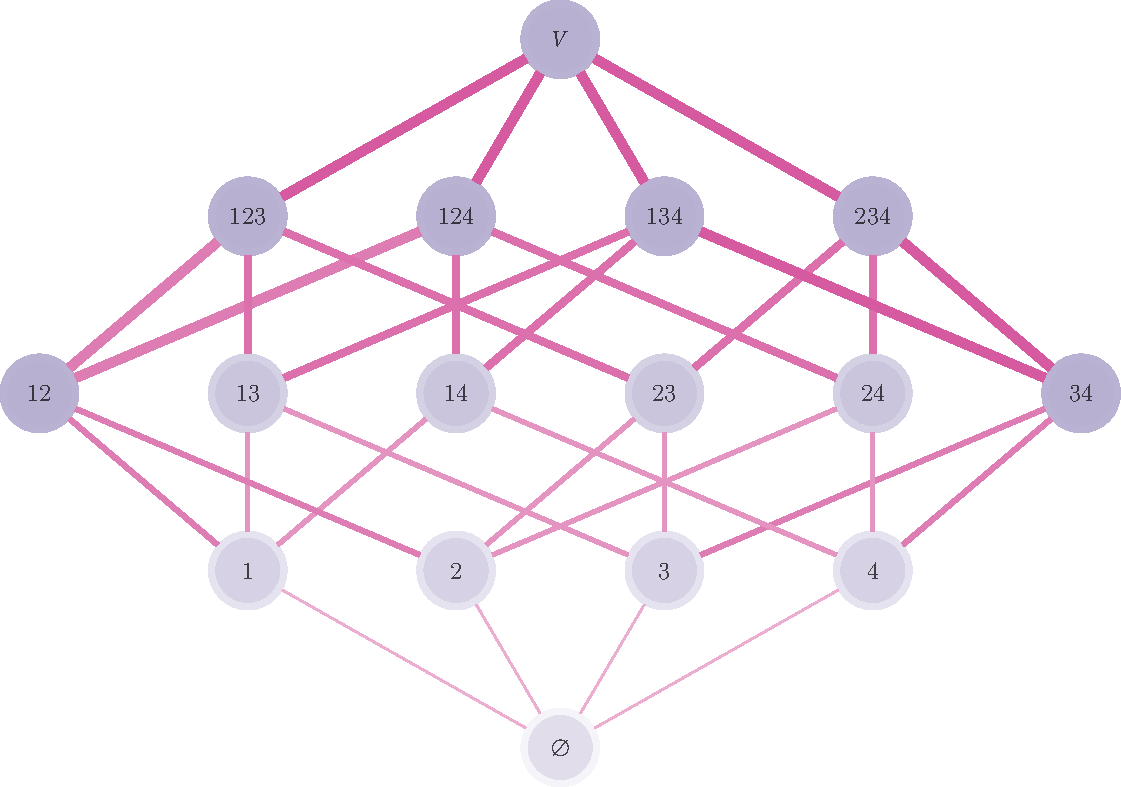
\includegraphics[width=\textwidth]{cp_easy_cong_end.pdf}\end{minipage}};
  \draw[LL] (f) to [out=-100,in=80] (a);
  \node[text=black,font=\sffamily,line width=1pt,draw=col1dark,fill=white,inner sep=4pt,rounded corners=2pt] (t1) at (1.1,1.7) {Theory};
  
  \node[NS] (b) at (2.8,0) {\begin{minipage}{8.5em}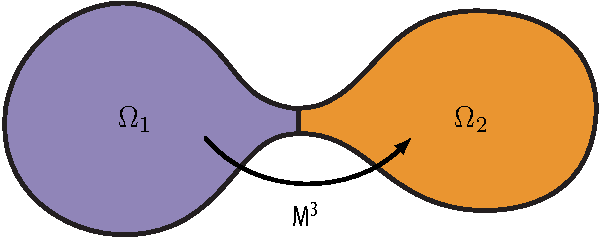
\includegraphics[width=\textwidth]{bottleneck3.pdf}\end{minipage}};
  \draw[LL] (f) to [out=-90,in=90] (b);
  \node[text=black,font=\sffamily,line width=1pt,draw=col1dark,fill=white,inner sep=4pt,rounded corners=2pt] (t1) at (2.8,1.7) {Algorithms};
  
  \begin{scope}[transparency group, opacity=0.0]
  \node[NS] (c) at (5.6,0) {\begin{minipage}{8.5em}\centering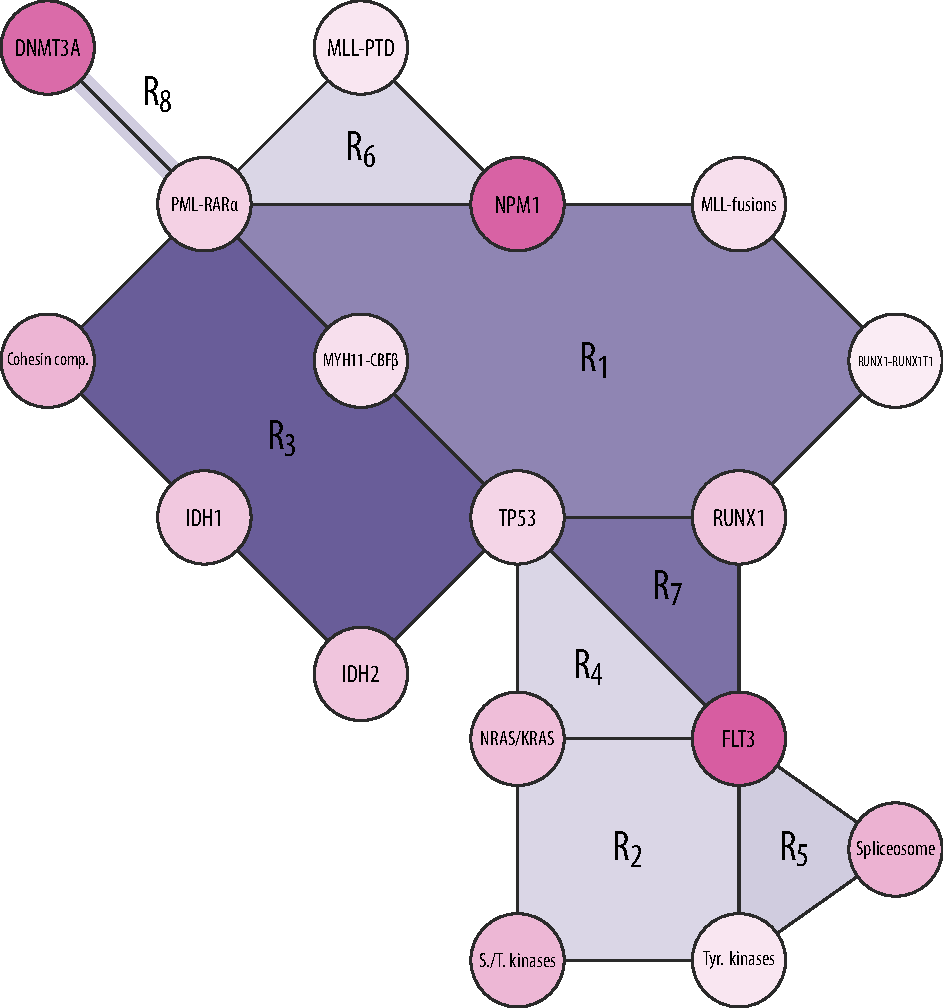
\includegraphics[width=0.7\textwidth]{graph_aml.pdf}\end{minipage}};
  \draw[LL] (f) to [out=-80,in=100] (c);
  \node[text=black,font=\sffamily,line width=1pt,draw=col1dark,fill=white,inner sep=4pt,rounded corners=2pt,rotate=0] (t1) at (4.5,1.7) {Applications};
  \end{scope}
\end{tikzpicture}

\end{document}